% ------------------------------------------------------------------------
% ------------------------------------------------------------------------
% ICMC: Modelo de Trabalho Acadêmico (tese de doutorado, dissertação de
% mestrado e trabalhos monográficos em geral) em conformidade com 
% ABNT NBR 14724:2011: Informação e documentação - Trabalhos acadêmicos -
% Apresentação
% ------------------------------------------------------------------------
% ------------------------------------------------------------------------

% Opções: 
%   Qualificação         = qualificacao 
%   Curso                = doutorado/mestrado
%   Situação do trabalho = pre-defesa/pos-defesa (exceto para qualificação)
% -- opções do pacote babel --
% Idioma padrão = brazil
	%french,	    	% idioma adicional para hifenização
	%spanish,			% idioma adicional para hifenização
	%english,			% idioma adicional para hifenização
	%brazil				% o último idioma é o principal do documento
\documentclass[brazil]{packages/icmc}

% Tag <hr> como comando \hr
\newcommand\hr{\par\vspace{-.5\ht\strutbox}\noindent\hrulefill\par}

% Comando simples para exibir comandos Latex no texto
\newcommand{\comando}[1]{\textbf{$\backslash$#1}}
% métodos em java
\newcommand{\method}[1]{\textit{#1}}

% ---
% Pacotes Opcionais
% ---
\usepackage{rotating}           % Usado para rotacionar o texto
\usepackage[all,knot,arc,import,poly]{xy}   % Pacote para desenhos gráficos
% Este pacote pode conflitar com outros pacotes gráficos como o ``pictex''
% Então é necessário usar apenas um dos pacotes conflitantes


% ---
% Informações de dados para CAPA e FOLHA DE ROSTO
% ---
\titulo{Algoritmo evolutivo para treinar um sistema inteligente para jogos de disputa}
\autor[Bastiani, L. G.]{Leonardo Guarnieri de Bastiani}
\orientador[Orientador:]{Prof. Dr.}{Eduardo do Valle Simões}
%\coorientador{Prof. Dr.}{Fulano de tal}
\curso{Engenharia de Computação}
\area{Computação Bioinspirada} % Área de concentração do trabalho
\data{08}{11}{2018} % Data do depósito
% ---


% ---
% RESUMOS
% ---

% Resumo em português
% conter no máximo 500 palavras
\newcommand{\fitness}{\textit{fitness}\xspace}
\textoresumo{
    Este trabalho trata do desenvolvimento de um algoritmo bioinspirado, composto por uma biblioteca e um estudo a partir dela, capaz de treinar um sistema inteligente para aprender a emular comportamento em jogos de disputa e de uma possível utilização desse algoritmo. Nos jogos do contexto deste algoritmo, há decisões a serem tomadas por dois jogadores, dependendo da situação de cada jogada. Para isso, o algoritmo evolutivo ajusta os parâmetros que são usados na tomada de decisão. Para o algoritmo, a função \fitness é a comparação dos resultados apresentados pelas soluções que forem sendo geradas para selecionar as mais adequadas para gerar novas alternativas de controladores.
    }{Computação bioinspirada, algoritmo evolutivo, aprendizado de máquina, gamificação}

% ---
% resumo em inglês
% ---
\textoresumo[english]{
    This project is about the development of a bioinspired algorithm capable of training an intelligent system to learn how to emulate behavior in dispute games and a possible use of this algorithm. In the games in the context of this algorithm, there are decisions to be made by two players, depending on the situation of each move. The evolutionary algorithm adjusts the parameters that are used in the decision making. The \fitness function is the comparison of the results presented by the solutions that are generated to select the most suitable ones to generate new alternatives of controllers.
    }{Bio-inspired computation, evolutionary algorithm, machine learning, gamification}
    
% ---
% Configurações de aparência do PDF final
% ---
% alterando o aspecto da cor azul
\definecolor{blue}{RGB}{41,5,195}

% informações do PDF
\makeatletter
\hypersetup{
     	pagebackref=true,
		pdftitle={\@title}, 
		pdfauthor={\@author},
    	pdfsubject={\imprimirpreambulo},
	    pdfcreator={LaTeX with abnTeX2/ICMC-USP},
		pdfkeywords={\palavraschave}, 
		colorlinks=true,       		% false: boxed links; true: colored links
    	linkcolor=blue,          	% color of internal links
    	citecolor=blue,        		% color of links to bibliography
    	filecolor=magenta,      	% color of file links
		urlcolor=blue,
		bookmarksdepth=4
}
\makeatother
% --- 

% ----------------------------------------------------------
% ELEMENTOS PRÉ-TEXTUAIS
% ----------------------------------------------------------

% Inserir a ficha catalográfica
%\incluifichacatalografica[tex/fichaCatalografica.pdf]
\incluifichacatalografica


% Inserir folha de aprovação
%
% Isto é um exemplo de Folha de aprovação, elemento obrigatório da NBR
% 14724/2011 (seção 4.2.1.3). Você pode utilizar este modelo até a aprovação
% do trabalho. Após isso, substitua todo o conteúdo deste arquivo por uma
% imagem da página assinada pela banca com o comando abaixo:
%
% \includepdf{folhadeaprovacao_final.pdf}
%
\begin{folhadeaprovacao}

  \begin{center}
    {\ABNTEXchapterfont\large\imprimirautor}

    \vspace*{\fill}\vspace*{\fill}
    {\ABNTEXchapterfont\bfseries\Large\imprimirtitulo}
    \vspace*{\fill}
    
    \hspace{.45\textwidth}
    \begin{minipage}{.5\textwidth}
        \imprimirpreambulo
    \end{minipage}%
    \vspace*{\fill}
   \end{center}
    
   Trabalho aprovado. \imprimirlocal, 24 de novembro de 2012:

   \assinatura{\textbf{\imprimirorientador} \\ Orientador} 
   \assinatura{\textbf{Professor} \\ Convidado 1}
   \assinatura{\textbf{Professor} \\ Convidado 2}
   %\assinatura{\textbf{Professor} \\ Convidado 3}
   %\assinatura{\textbf{Professor} \\ Convidado 4}
      
   \begin{center}
    \vspace*{0.5cm}
    {\large\imprimirlocal}
    \par
    {\large\imprimirdata}
    \vspace*{1cm}
  \end{center}
  
\end{folhadeaprovacao}
% ---

% DEDICATÓRIA / AGRADECIMENTO / EPÍGRAFE
\textodedicatoria*{tex/pre-textual/dedicatoria}
\textoagradecimentos*{tex/pre-textual/agradecimentos}
\textoepigrafe*{tex/pre-textual/epigrafe}

% Inclui a lista de figuras
\incluilistadefiguras

% Inclui a lista de tabelas
%\incluilistadetabelas

% Inclui a lista de quadros
%\incluilistadequadros

% Inclui a lista de algoritmos
\incluilistadealgoritmos

% Inclui a lista de códigos
%\incluilistadecodigos

% Inclui a lista de siglas e abreviaturas
\incluilistadesiglas

% Inclui a lista de símbolos
%\incluilistadesimbolos

% ----
% Início do documento
% ----
\begin{document}

% ----------------------------------------------------------
% ELEMENTOS TEXTUAIS
% ----------------------------------------------------------
\textual

\chapter{Introdução}
\label{chapter:introducao}
\section{Motivação e Contextualização}

\newcommand\SE{\sigla{SE}{Sistema Evolutivo}\xspace}

Este trabalho relata a criação de uma biblioteca que aplica os conceitos de Computação Bioinspirada e sua aplicação em um sistema desconhecido com entradas e saídas bem definidas. O uso de algoritmos evolutivos é um contraste de algoritmos determinísticos  e incorporam outro viés de solução por um \SE\cite{Layzell1999} para ajustar continuamente os parâmetros de controlador às variações na configuração do ambiente de trabalho.

A área de pesquisa conhecida como Computação Bioinspirada procura encontrar soluções elegantes e eficientes que resolvem problemas grandes que poderiam demandar tempo computacional incompatível com a necessidade de resposta através de técnicas tradicionais. O comportamento social de formigas e abelhas, estratégia de caça de predadores ou o ciclo de atividade e hibernação de ursos são modelos e inspirações para essa área, estes exemplos ilustram soluções de problemas que podem incluir otimização, orientação e reconhecimento de padrões, tudo isso sendo obtido através de um processo evolutivo.\footnote{Simões, E. D. V. (2000). Indelevelmente Of An Embedded Evolutionary Controller To Enable Collision-Free Navigation Of A Population Of Autonomous Robots. University of Kent at Canterbury, Inglaterra p. 289}

A técnica estudada neste trabalho denomina-se Computação Evolutiva da calsse de técnicas conhecida como Computação Biológica ou Biocomputação que se inspira em princípios biológicos para projetar o algoritmo computacional, mais especificamente no comportamento social de organismos.

Um algoritmo evolutivo é capaz de caminhar a solução de um problema através da comparação de uma função \fitness que é uma função de comparação entre duas soluções. Por tanto, nesse trabalho, a ferramenta desenvolvida tem sua função \fitness como a comparação entre duas entidades que competem, o vencedor é aquele com uma melhor função \fitness. Foi estudada uma aplicação desse algoritmo com a comparação entre um sistema qualquer com entradas e respostas de modo a prever as possíveis respostas do sistema.

\section{Objetivos}

Este trabalho visa desenvolver uma biblioteca de algoritmo evolutivo que se enquadra em situações onde pode-se comparar duas soluções por meio de disputas capaz de se adaptar às alterações de cada cenário e estudar sua aplicação em um sistema com entradas e saídas bem definidas de modo a prever novas saídas.

A biblioteca implementa os conceitos de Indivíduo, que é um dos participantes de uma disputa, e de Gene, que é um dos fatores que determinará como um indivíduo responde a uma entrada. Nos estudos da utilização dessa ferramenta, foram feitos sistemas com saídas que seguem uma determinada lógica e os resultados foram comparados com um sistema que gera saídas aleatoriamente.

\section{Organização}

Este documento relata os métodos desenvolvidos e aplicados para a construção do algoritmo, além de citar fontes que comprovam a eficácia e estudos com aplicações do algoritmo que o validam.

O código-fonte produzido para essa aplicação está disponibilizado\footnote{\url{https://github.com/leobastiani/AE}} e uso da biblioteca para novas ferramentas que podem ser modeladas nos casos propostos, isto é, que são capazes de realizar disputas entre dois, gerando um melhor vencedor e um perdedor.


\chapter{Métodos, Técnicas e Tecnologias Utilizadas}
\label{chapter:metodos}
\section{Revisão Bibliográfica} \label{secao:rev_bib}

A inspiração do paradigma da Computação Evolutiva vem da evolução natural formalizada por Darwin \cite{Ridley1996}. Algoritmos embebidos desta tese possuem passos genéricos capazes de resolver um grande número de problemas práticos, e possuem características como auto-organização e comportamento adaptativo \cite{Goldberg1988}, portanto são capazes de tratar problemas computacionalmente complexos com uma ferramenta de propósito geral. Por outro lado, esses algoritmos não garantem a obtenção de uma solução ótima \cite{Zuben2000} por poder convergir para soluções localmente ótimas.

A linguagem de programação Java foi escolhida para a criação da ferramenta, os motivos para essa escolha foram:

\newcommand{\JVM}{\sigla{JVM}{Java Virtual Machine}\xspace}

\begin{itemize}
    \item Multiplataforma: Java é uma linguagem capaz de ser executada em qualquer sistema que possua uma \JVM, sua execução e desenvolvimento independe do sistema, permitindo que a aplicação desenvolvida não sofra essa restrição.
    \item Desempenho: entre as linguagens de programação que são interpretadas, Java possui um desempenho melhor por ser compilada e interpretada, gerando um código intermediário que é executado pela \JVM.
    \item Facilidade e didática: Java é uma linguagem que permite certas comodidades ao programador com um bom balanço de desempenho, como a ferramenta desenvolvida foi utilizada para estudos e é de uso genérico, as facilidades fornecidas pela linguagem são importante para agilizar e pela validação do trabalho.
    \item Modelagem: a modelagem de classes fornecida por Java ajudam no entendimento e no reuso da biblioteca desenvolvida.
\end{itemize}

Nesse projeto há uma contextualização do problema nos seguintes moldes:

\begin{itemize}
    \item Indivíduo: um indivíduo é a representação de um jogador que possui uma pontuação provida da função \fitness de acordo com as respostas produzidas por esse jogador.
    \item Gene: um gene é uma entidade capaz de provocar uma resposta. Para cada tipo de respostas há um grupo de genes. As entradas de um sistema são capazes de excitar o gene e o gene mais excitado responde pelo indivíduo.
    \item Disputa: é uma função entre dois indivíduos que gera um vencedor e um perdedor com base na função \fitness. Uma disputa deve necessariamente retornar o quão melhor um indivíduo foi em relação a outro.
\end{itemize}

Por tanto, o indivíduo que possui os melhores genes terá uma função \fitness melhor e ganhará mais disputas.

\section{Algoritmos evolutivos}
Os algoritmos evolutivos podem ser resumidos em um roteiro básico de procedimentos \cite{Todd1997} que são adaptados de acordo com o contexto do problema a ser solucionado \cite{Werger1999} \cite{Mitchell1995}. Um algoritmo evolutivo é usualmente composto por:

\newcommand{\crossover}{\textit{crossover}\xspace}

\begin{itemize}
    \item Representação de genes dos indivíduos: Biologicamente, cada gene representa uma característica do indivíduo, e o cromossomo, que é o conjunto de genes de um indivíduo, representa o indivíduo. Computacionalmente, o cromossomo representa um candidato à solução do problema e o gene representa uma função para obtenção de uma resposta.
    \item Função \fitness (ou de adaptação): indica, para cada indivíduo, o valor de aptidão, mostrando a aproximação da solução proposta pelo indivíduo em relação à solução procurada.
    \item Função de reprodução: Determina novos indivíduos que representarão a próxima geração da população do algoritmo herdando características que são encontradas nos indivíduos com uma maior função \fitness (ou mais aptos), propagando seus genes. O \crossover e mutações ocorrem na função de reprodução, de modo análogo ao biológico.
\end{itemize}

Em um algoritmo evolutivo, a população inicial é constituída por indivíduos com genes aleatórios, ou seja, o início do algoritmo parte de uma solução aleatória e a cada geração, o valor de \fitness ou adequação é calculado em cada indivíduo. A função de reprodução gera novos indivíduos e as características positivas de cada indivíduo podem ser propagadas para a nova geração, assim a solução caminha para uma resposta adequada. O fluxograma na Figura \ref{figura:fluxograma_ae} representa estas etapas.

\begin{figure}[htb]
    \caption{Fluxograma de uma implementação típica de um algoritmo evolutivo.}
    \label{figura:fluxograma_ae}
    \centering
    %scale=0.8
    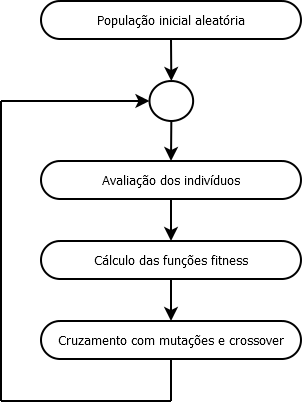
\includegraphics[scale=1]{images/dia/fluxograma-ae}
    \fautor
\end{figure}

\chapter{Desenvolvimento}
\label{chapter:desenvolvimento}
\section{O Problema}

O projeto consiste do desenvolvimento de uma biblioteca de algoritmo evolutivo genérica para solucionar problemas com gamificação de disputas, ou seja, encontrar soluções que possam ser comparadas através de uma disputa entre dois jogadores, gerando um vencedor e um perdedor necessariamente. Bem como estudar as aplicações desse algoritmo em um sistema com entradas e saídas bem definidas, de modo que a solução não esteja implícita em nenhuma das entradas e saídas, mas que o algoritmo possa evoluir livremente para encontrar o melhor rearranjo dos genes até produzir respostas idênticas as oferecidas pelo sistema.

\section{Biblioteca de Algoritmos Evolutivos}

Foi feita uma biblioteca para uso de algoritmos evolutivos em Java que emprega os conceitos de Indivíduos e Genes. Para aplicações diferentes das estudadas nesse documento, a biblioteca ainda pode ser usada em qualquer \SE, pois pode ser estendida e rearranjada para qualquer aplicação dentro desse conceito. As classes e métodos implementadas pela biblioteca estão descritas a seguir.

\subsection{Classe AE}

Esta classe é responsável por englobar as funções referentes ao algoritmo evolutivo em si, ou seja, ela organiza e remaneja os indivíduos, realiza confrontos, compara soluções, seleciona os melhores e recombina os indivíduos de modo que as melhores soluções propaguem suas características.

As disputas realizadas pelos indivíduos seguem um sistema de torneio mata-mata\footnote{\url{https://pt.wikipedia.org/wiki/Competições_eliminatórias}}, que por padrão possui 16 participantes, no qual o primeiro e segundo colocados cruzam suas características genéticas com os indivíduos que não foram enfrentados por eles.

\begin{figure}[htb]
    \caption{Torneio realizado pela classe AE. A ilustração demonstra um caso em que o campeão do torneio veio dos indivíduos de 0 a 7 e o vice-campeão veio dos indivíduos de 8 a 15.}
    \label{figura:funcao_playAll}
    \centering
    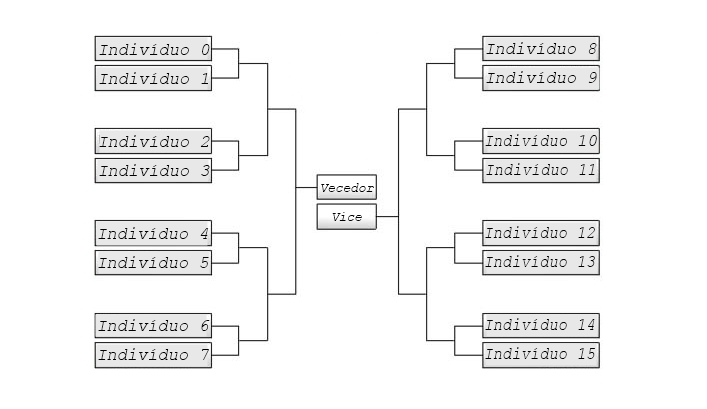
\includegraphics[scale=0.8]{images/ps/mata-mata}
    \fautor
\end{figure}

Neste torneio, há dois grupos, o grupo da esquerda composto pelos indivíduos de 0 a 7 e o grupo da direita composto pelos indivíduos de 8 a 15. O campeão do torneio transmite os genes para o grupo em que não obteve confrontos, com exceção do vice-campeão, e o mesmo ocorre para o vice-campeão.

A Figura \ref{figura:funcao_playAll} demonstra como funciona esse torneio e a propagação das características dos melhores colocados, exemplificando que o indivíduo campeão estava entre os indivíduos de 0 a 7 e o vice-campeão estava entre os indivíduos de 8 a 15, sendo assim, o campeão transmite suas características genéticas para os indivíduos de 8 a 15, com exceção do vice-campeão, e vice-versa.

A classe AE possui outras funções implementadas que são de uso diverso e serão discutidas em outra subseção.

\subsection{Classe Eq}

\newcommand{\var}[1]{\textit{#1}}

A classe Eq representa uma equação e possui uma função como representa a equação \ref{eq:eq}. Onde as variáveis \var{factor} e \var{sum} correspondem a variáveis internas da classe e constituem parte de um gene.

\begin{equation}
    \label{eq:eq}
    f(x)=\mathrm{factor}*x + \mathrm{sum}
\end{equation}

\subsection{Classe Indivíduo}

A classe indivíduo representa um indivíduo capaz de gerar uma solução para o sistema. A função \fitness de cada indivíduo é responsável por informar o quão boa é a solução deste indivíduo. Se um indivíduo ganha mais confrontos do que outro, sua função \fitness será maior.

Na biblioteca, o indivíduo possui o método \method{play} que recebe outro indivíduo como parâmetro. O usuário escolhe como confrontar os dois indivíduos retornando 0 se o vencedor for indivíduo que chama o método, ou 1, se o vencedor for o indivíduo referenciado no parâmetro. Nesta função não é possível retornar uma informação para os casos de empate. Como este projeto foca uma disputa entre dois indivíduos, o método \method{play} pode confrontar esses dois indivíduos $N$ vezes e basear sua função \fitness na quantidade de partidas vencidas, além de retornar o indivíduo que mais venceu partidas como vitorioso.

\subsection{Classe Gene}

Cada indivíduo pode possuir uma determinada quantidade de genes que são capazes de gerar uma resposta. O gene pode ser excitado de alguma forma pelo sistema e possui um valor de estado que pode aumentar de acordo com a operação operação de consumir um estado. Portanto um gene possui duas funções que envolvem a variável \var{estado}:

\begin{itemize}
    \item \method{Consumir}: O método de \method{consumir} altera a variável \var{estado} do gene conforme a equação \ref{eq:gene_consumir} onde $x$ é o valor da entrada, $i$ é a posição da entrada no ventor de entradas de um sistema, ou seja, se um sistema possui entradas com vetor de tamanho $N$, $i$ terá valores de 0 até $N-1$, $E$ e $I$ são funções descritas em \ref{eq:eq}.
    \begin{equation}
        \label{eq:gene_consumir}
        \mathrm{Estado} \leftarrow \mathrm{Estado} +  E(x) * I_i(i)
    \end{equation}
    \item \method{Reset}: O método de \method{reset} devolve o \var{estado} do gene para um estado inicial. A classe Gene possui as variáveis internas \var{estado}, \var{estadoInicial}, \var{limiteSup} e \var{limiteInf}. A função de \method{reset} está descrita no algoritmo \ref{algoritmo:gene_reset}.
\end{itemize}

\begin{algoritmo}
\caption{Algoritmo de reinicio de gene.}
\label{algoritmo:gene_reset}
    \If(\tcp*[f]{Se o estado do gene está fora dos limites})
    {estado > limiteSup {\normalfont \textbf{or}} estado < limiteInf} {
        $estado \gets estadoInicial$
    }
\end{algoritmo}

\subsection{Outras implementações} \label{secao:vetor_estados}

A biblioteca implementa outras funções que são necessárias para a execução do \SE e facilitam o trabalho de desenvolvedores que a utilizam, elas são:

\begin{itemize}
    \item Funções para gerar números aleatórios:
        \begin{itemize}
            \item Funções para gerar números aleatórios inteiros ou com ponto decimal;
            \item Função para gerar números aleatórios com média deslocada para as bordas, pois a solução pode ter uma combinação de valores bem distinta.
        \end{itemize}
    \item Cruzamento de números: esta função realiza um sorteio com as possibilidades de:
        \begin{itemize}
            \item Manter o valor que estava;
            \item Adquirir o valor da melhor solução;
            \item Definir o novo valor como a média entre a melhor solução e o valor atual.
        \end{itemize}
    \item Uma classe de estados: como esse projeto tem uma área dedicada ao estudo de previsão de estados, que é um sistema com entradas e saídas bem definidas, a classe de estados implementada para essa solução foi mantida no projeto de biblioteca para um \SE.
    \item Descarte dos piores genes: a fim de aumentar a variabilidade genética, há um parâmetro que configura o número de gerações para que ocorra um descarte dos piores indivíduos por novos.
\end{itemize}

Esse conjunto de funções extra traduz que uso da biblioteca em outros projetos gera um aumento de produtividade e diminuição do tempo necessário para a conclusão.

\subsection{Resultados}

A biblioteca produzida pode ser aplicada para quaisquer situações em que pode-se abstrair uma solução baseada em disputas de dois jogadores. Por outro lado, essa biblioteca encara a função \fitness do algoritmo evolutivo de outra forma, o melhor algoritmo é aquele capaz de vencer mais jogos.

Outro fator importante para o sucesso da biblioteca é o fator de que os indivíduos que não foram confrontados são aqueles que recebem as característica do melhor. Assim, cria-se a lógica de que as estratégias tomadas por um dos indivíduos passará para o outro ramo de jogadores. Por tanto, se houver duas boas estratégias de jogo, as duas se enfrentarão em várias etapas e os melhores indivíduos propagarão sua estratégia para outro ramo que enfrenta um dos melhores, mas com outra estratégia.

A biblioteca facilita o desenvolvimento de programas que necessitam de um \SE por já estar implementada e testada. Qualquer usuário pode reutilizar a biblioteca, pois ela é de código aberto e está disponibilizada através da plataforma GitHub\footnote{Disponível em \url{https://github.com/leobastiani/AE}}. Além disso, a biblioteca implementa alguns conceitos no \SE que guiam o pensamento do desenvolvedor.

\section{Algoritmo evolutivo para previsão de estados}

Foi feito um estudo utilizando a biblioteca desenvolvida nesse projeto a fim de criar um sistema que recebe um vetor de Estado e é capaz de prever os resultados dos estados de saída baseado nas entradas.

O vetor de estados é uma classe que possui um vetor de entradas e um vetor de saídas, mas as saídas são bem definidas, ou seja, seguem um número limitado que vai de 0 até $N-1$, sendo o $N$ o número de saídas possíveis.

Para esse projeto, foi feito um estudos com saídas de tamanho $N=3$, um número relativamente pequeno, mas que pode representar muitas situações, como casos de uma previsão de vitória, derrota ou empate. Além disso, um número de saídas pequeno diminui o tempo de convergência do algoritmo evolutivo, permitindo que vários testes possam ocorrer e várias alterações de melhorias puderam ser tomadas durante o tempo de produção desse projeto.

A biblioteca produzida foi estendida e utilizada, as alterações feitas para o uso da biblioteca estão detalhadas a seguir.

\subsection{Classe Indivíduo}

Um indivíduo recebe as entradas do sistema e a cada iteração, produz uma saída de acordo com os valores de estado de seus genes. Um bom individuo é aquele capaz de prever as saídas dos estados dependendo das entradas. O melhor indivíduo é aquele que prevê todas saídas.

Os confrontos entre indivíduos se dão do seguinte critério:
\begin{itemize}
    \item Comparação entre o número de acertos: os indivíduos que mais acertaram estados de saídas são considerados melhores do que indivíduos que acertaram menos.
    \item Comparação entre a segunda hipótese de saída: os indivíduos que não acertaram o estado, mas que deixaram a saída correta como segunda opção ficam melhores posicionados do que os indivíduos que também não acertaram, mas que também não consideraram a saída correta como segunda hipótese.
\end{itemize}

Paralelamente, os indivíduos possuem uma função de pontuação que aumenta em 1 quando um indivíduo acerta uma resposta como primeira alternativa, e aumenta em 0,5 quando um indivíduo acerta a resposta como segunda alternativa.

\subsection{Classe Resposta de Gene}

Essa classe é uma extensão da classe Gene, acrescentando as seguintes funcionalidades:
\begin{itemize}
    \item Conter mais genes consecutivos: cada gene forma uma lista encadeada com outro gene.
    \item Cada gene possui uma informação de resposta: as respostas possíveis de cada gene variam de 0 até $N-1$.
\end{itemize}

Mas essa classe segue as mesmas regras da classe Gene, ou seja, o Gene mais excitado é considerado como a resposta do indivíduo.

\subsection{Estados do sistema analisados}

Entre os possíveis estados para se analisar, a melhor escolha foi um sistema de vetor de entradas $E$ de tamanho 3 e vetor de saídas $S$ de tamanho 1 descrito por:

\begin{gather*}
    2 \quad \mathrm{se} \quad E_2 > E_0 \quad \mathbf{e} \quad E_2 > E_1 \\
    1 \quad \mathrm{se} \quad \sum E_1 > \sum E_0 \\
    0 \quad \mathrm{c.c.}
\end{gather*}

Esse sistema é um bom caso de estudo pois:

\begin{itemize}
    \item Possui fatores acumulativos: a resposta do sistema depende de uma memória, ou seja, o estado anterior influencia na próxima resposta.
    \item Possui fatores situacionais: a resposta do sistema depende de uma situação momentânea, ou seja, para determinadas entradas, a resposta descarta uma lógica.
    \item Possui muitas comparações: o sistema faz várias comparações e o algoritmo evolutivo deve imitar ou simular as comparações para obter as respostas.
\end{itemize}

Os valores de entrada foram obtidos aleatoriamente e foram feitos teste com 200 e 100 estados, mas o há uma condição, o número de saídas de um valor de resposta deve ser de no mínimo um quinto do número de estados, isso foi determinado para que houvesse uma quantidade razoável de todas as respostas possíveis. Testes com 200 estados produziram resultados semelhantes aos testes com 100 estados, porém o algoritmo necessita de mais tempo para convergir, por isso, o daremos foco com testes de 100 estados.

\subsection{Resultados}

Os resultados variam de acordo com a amostragem, porém as taxas de acerto obtida pelo algoritmo foram melhores do que tentativas aleatórias.

O conjunto 1 de estados produziu uma resposta com taxa de acerto de 96 dentre os 100, com 97,5 pontos. Nesse caso, o indivíduo com melhor resposta possui 4 genes, 2 genes destinas a resposta 2 e as demais respostas com apenas 1 gene. Para esse mesmo conjunto de estados, mas com obtenção de genes aleatórios, o melhor indivíduo encontrado após o mesmo número de gerações obteve 72 acertos com 84,5 pontos. A convergência do algoritmo ocorreu aproximadamente com 50.000 gerações. A Figura \ref{figura:resultado_97} mostra a evolução da função \fitness.

\begin{figure}[htb]
    \caption{Histórico de \fitness do conjunto 1 de estados.}
    \label{figura:resultado_97}
    \centering
    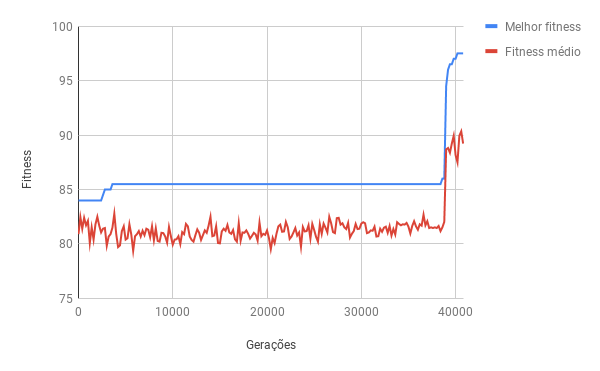
\includegraphics[scale=0.8]{images/resultado_97}
    \fautor
\end{figure}

Outro conjunto 2 de estados obteve uma resposta com taxa de acerto de 79 de 100 e 86,5 pontos. Nesse caso, o indivíduo com melhor resposta possui 4 genes, 2 genes destinas a resposta 0 e as demais respostas com apenas 1 gene. Apesar desse conjunto ter uma resposta muito inferior ao conjunto 1, ainda assim, o algoritmo evolutivo foi melhor do que uma tentativa de genes aleatórios, que obtiveram 77 acertos com 84 pontos. Ambos os resultados foram obtidos com aproximadamente 70.000 gerações. A Figura \ref{figura:resultado_79} mostra a evolução da função \fitness.

\begin{figure}[htb]
    \caption{Histórico de \fitness do conjunto 2 de estados.}
    \label{figura:resultado_79}
    \centering
    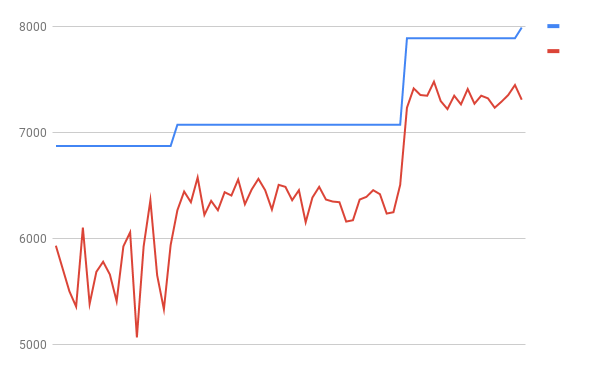
\includegraphics[scale=0.8]{images/resultado_79}
    \fautor
\end{figure}

Outros 10 conjuntos de estados foram analisados, a Figura \ref{figura:dez_execucoes} há resultados de execuções do algoritmo após 100.000 gerações, comparando o melhor indivíduo obtido pelo algoritmo com o melhor indivíduo obtido aleatoriamente, a figura mostra que o algoritmo obteve uma pontuação melhor do que tentativas aleatórias de acerto em todos os casos, evidenciando que o algoritmo caminha de alguma forma para uma solução.

\begin{figure}[htb]
    \caption{Resultado de dez execuções do algoritmo com 100.000 gerações comparando o melhor indivíduo obtido pela lógica da biblioteca com outro obtido aleatoriamente}
    \label{figura:dez_execucoes}
    \centering
    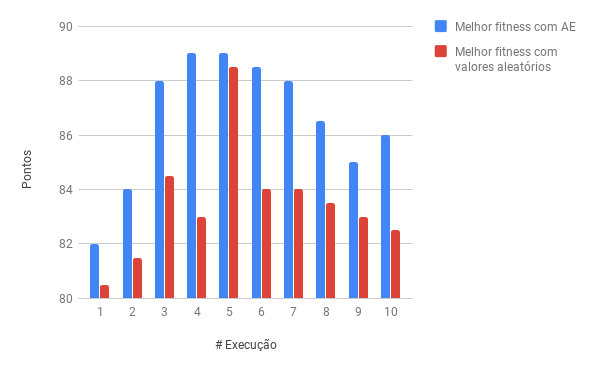
\includegraphics[scale=0.8]{images/dez_execucoes}
    \fautor
\end{figure}

\section{Dificuldades e Limitações}

\subsection{Sobre a biblioteca desenvolvida}

A biblioteca está implementada nos moldes citados e testada, entretanto, limita o usuário a linguagem Java. Idealmente a biblioteca deveria ser escrita em C/C++, compilada como executável de biblioteca dinâmica e adaptada para as mais diversas linguagens do mercado, essas mudanças ajudariam no desempenho e no reuso da biblioteca para outras linguagens. O projeto não foi desenvolvido dessa maneira pelas vantagens citadas na seção \ref{secao:rev_bib}, por se tratar de um material de estudo, os benefícios de Java foram importantes para o projetista.

\subsection{Sobre o algoritmo evolutivo para previsão de estados}

Os testes aplicados a esse estudos obtiveram resultados melhores do que vetores aleatórios, mas se demonstraram dependentes dos valores fornecidos. Em situações com uma amostragem de dados muito grande, é possível selecionar os melhores dados para alimentar o algoritmo evolutivo a fim de se encontrar os melhores parâmetros para previsão.

Os testes realizados foram com poucas entradas e com poucas saídas definidas, devido ao tempo computacional requerido para muitas entradas ou muitas saídas. Esse tema será discutido na seção de trabalhos futuros.

Embora os Algoritmos Evolutivos tenham sido exaustivamente explorados no meio acadêmico, os mesmos encontram resistência para serem aceitos no desenvolvimento de certas aplicações como jogos, devido ao fato de pesquisadores apontarem a técnica como lenta e capaz de permitir a obtenção de desempenhos ruins \cite{Sweetser2002} \cite{Spronck2003} \cite{Marcio2008}. Neste trabalho, os resultados não foram surpreendentes, são dependentes das entradas e análises com muitas entradas provocam lentidão.

\chapter{Conclusão}
\label{chapter:conclusao}
O algoritmo desenvolvido pode ser aplicado para diversas áreas da computação bio-inspirada e acrescenta um novo conceito sobre funções \fitness. A função \fitness pode ser obtida em casos de disputa entre dois jogadores comparando o desempenho entre eles numa disputa.

% \chapter{Citações e Referências}
% \label{chapter:citacoes}
% Em documentos acadêmicos podem existir citações diretas e citações indiretas. As citações indiretas são feitas quando se reescreve uma referência consultada. Nas citações indiretas há duas formatações possíveis dependendo de como ocorre a citação no texto. Quando o autor é mencionado explicitamente  deve ser usado o comando \comando{citeonline\{\}}, nas demais situações é usado o comando \comando{cite\{\}}. No quadro \ref{figura:citacao_indireta_explicita} encontrasse um  exemplo de uso do comando \comando{citeonline\{\}}.

\begin{quadro}[htb]
\caption{Exemplo de citação indireta explícita} \label{figura:citacao_indireta_explicita}
\hrulefill

\lstset{language=Tex, breaklines=true}
\begin{lstlisting}
Segundo \citeonline{silveira:2006}, o trabalho de conclusão de curso deve seguir as normas da ABNT.
\end{lstlisting}

\hrulefill

Segundo \citeonline{silveira:2006:manual_tcc}, o trabalho de conclusão de curso deve seguir as normas da ABNT.

\hrulefill

%\legend{Fonte: o autor.}
\end{quadro}

Para especificar a página consultada na referência é preciso acrescentá-la entre colchetes com os comandos \comando{cite[página]\{\}} ou \comando{citeonline[página]\{\}}. No quadro \ref{figura:citacao_indireta_pagina} é mostrado um exemplo de citação com página específica.

\begin{quadro}[htb]
\caption{Exemplo de citação indireta não explícita} \label{figura:citacao_indireta_pagina}
\hrulefill

\lstset{language=Tex, breaklines=true}
\begin{lstlisting}
A folha de aprovação é um elemento obrigatório na monografia de projeto final de curso trabalho de conclusão de curso.  \cite[p.~10]{silveira:2006}.
\end{lstlisting}

\hrulefill

A folha de aprovação é um elemento obrigatório no trabalho de conclusão de curso.  \cite[p.~10]{silveira:2006:manual_tcc}.

\hrulefill

\end{quadro}

As citações diretas acontecem quando o texto de uma referência é transcrito literalmente. As citações diretas são curtas (até três linhas) são inseridas no texto entre aspas duplas. Conforme exemplo no quadro \ref{figura:citacao_direta_curta}.

\begin{quadro}[htb]
\caption{Exemplo de citação direta curta}
\label{figura:citacao_direta_curta}
\hrulefill

\lstset{language=Tex, breaklines=true}
\begin{lstlisting}
``Os quadros, ao contrário das tabelas, apresentam dados textuais e devem localizar-se o mais próximo do texto a que se referem'' \cite[p.~25]{silveira:2006}.
\end{lstlisting}

\hrulefill

``Os quadros, ao contrário das tabelas, apresentam dados textuais e devem localizar-se o mais próximo do texto a que se referem'' \cite[p.~25]{silveira:2006:manual_tcc}.

\hrulefill
\end{quadro}

As citações longas (com mais de 3 linhas) podem ser inseridas via \comando{begin\{citacao\}} conforme quadro \ref{figura:citacao_direta_longa}.

\begin{quadro}[htb]
\caption{Exemplo de citação direta longa}
\label{figura:citacao_direta_longa}
\hrulefill

\lstset{language=Tex, breaklines=true}
\begin{lstlisting}
\begin{citacao}
Síntese final do trabalho, a conclusão constitui-se de uma resposta à hipótese enunciada na introdução. O autor manifestará seu ponto de vista sobre os resultados obtidos e sobre o alcance dos mesmos. Não se permite a inclusão de dados novos nesse capítulo nem citações ou interpretações de outros autores \cite[p.~25]{silveira:2006}.
\end{citacao}
\end{lstlisting}

\hrulefill

\begin{citacao}
Síntese final do trabalho, a conclusão constitui-se de uma resposta à hipótese enunciada na introdução. O autor manifestará seu ponto de vista sobre os resultados obtidos e sobre o alcance dos mesmos. Não se permite a inclusão de dados novos nesse capítulo nem citações ou interpretações de outros autores \cite[p.~25]{silveira:2006:manual_tcc}.
\end{citacao}

\hrulefill

\end{quadro}


% ---
% Finaliza a parte no bookmark do PDF, para que se inicie o bookmark na raiz
% ---
\bookmarksetup{startatroot}% 
% ---

% ----------------------------------------------------------
% ELEMENTOS PÓS-TEXTUAIS
% ----------------------------------------------------------
\postextual

% ----------------------------------------------------------
% Referências bibliográficas
% ----------------------------------------------------------
\bibliography{references}

% ---------------------------------------------------------------------
% GLOSSÁRIO
% ---------------------------------------------------------------------

% Arquivo que contém as definições que vão aparecer no glossário
\newword{30}{Função fitness}{Função que pode medir o quão boa é uma solução em uma escala numérica}

\newword{35}{Java}{Linguagem de programação orientada a objetos que gera um \textit{bytecode} para ser interpretado pela JVM, portanto, é uma linguagem semi-compilada, trazendo benefícios de linguagens compiladas e interpretadas}

\newword{36}{Java Virtual Machine}{JVM é uma máquina virtual que possibilita um computador executar programas em Java}


% Comando para incluir todas as definições do arquivo glossario.tex
\glsaddall
% Impressão do glossário
\printglossaries

% ----------------------------------------------------------
% Apêndices
% ----------------------------------------------------------

% ---
% Inicia os apêndices
% ---
% \begin{apendicesenv}

%     \chapter{Documento Básico Usando a Classe icmc}
%     \label{chapter:documento-basico}
%     
\begin{codigo}[caption={Exemplo de um documento básico}, label={codigo:documento-basico}, language=Tex, breaklines=true]
% Documento utilizando a classe ufgcac
% Opções: 
%   Qualificação         = qualificacao 
%   Curso                = doutorado/mestrado
%   Situação do trabalho = pre-defesa/pos-defesa (exceto para qualificação)
% -- opções do pacote babel --
% Idioma padrão = brazil
	%french,	    % idioma adicional para hifenização
	%spanish,			% idioma adicional para hifenização
	%english,			% idioma adicional para hifenização
	%brazil				% o último idioma é o principal do documento
\ documentclass[doutorado, spanish, english, brazil]{packages/icmc}

% Título do trabalho
\titulo{Título da Monografia}

% Nome do autor
\autor[Abreviação]{Nome completo do autor}

% Define o local
\local{São Carlos -- SP}

% Data do depósito
\data{18}{12}{2012}

% Nome do Orientador
\orientador[Orientador:]{Titulação do orientador}{Nome completo do Orientador}

% Nome do Coorientador (caso não exista basta remover)
\coorientador[Coorientador:]{Titulação do coorientador}{Nome completo do Coorientador}
% Se coorientadora troque Coorientador: por Coorientadora: dentro do colchetes

% Define o nome da instituição
\instituicao{Instituto de Ciências Matemáticas e de Computação (ICMC/USP)}

% Especiolidade e Nome do programa de Pós-graduação
\curso[Ciências -- Ciências de Computação e Matemática Computacional]{Ciências de Computação e Matemática Computacional}
% O valor entre colchetes é opcional

% Resumo
\textoresumo[Idioma]{
Texto do resumo do trabalho.
}{Lista de palavras-chave separada por virgulas}


% Início do documento
\begin{document}

\chapter{Introdução}

Capítulo de Introdução

\chapter{Desenvolvimento}

Capítulo de Desenvolvimento

\chapter{Conclusão}

Capítulo de conclusão

% Nome do arquivo com as referências bibliográficas
\bibliography{referencias}

\end{document}

\end{codigo}

% \end{apendicesenv}
% ---


% ----------------------------------------------------------
% Anexos
% ----------------------------------------------------------

% ---
% Inicia os anexos
% ---
% \begin{anexosenv}

%     \chapter{Páginas Interessantes na Internet} 
%     \label{chapter:paginas-interessantes}
%     \begin{description}
 \item[\url{http://www.tex-br.org}]: Página em português com diversos tutoriais e referências interessantes sobre \LaTeX;
 \item[\url{http://en.wikibooks.org/wiki/LaTeX}]: Livro em formato \textit{wiki} gratuito sobre \LaTeX;
 \item[\url{http://tobi.oetiker.ch/lshort/lshort.pdf}]: Ótimo tutorial sobre \LaTeX (possui versão em português \url{http://alfarrabio.di.uminho.pt/~albie/lshort/ptlshort.pdf}, mas a versão em inglês é a mais atual);
 \item[\url{http://code.google.com/p/abntex2/}]: Página do abnTeX2, grupo que desenvolve os pacotes e classes em \LaTeX para as normas da ABNT, nos quais a classe \textit{icmc} foi baseada;
\item[\url{ http://www.rexlab.ufsc.br:8080/more/index.jsp}]: Página do Mecanismo On-line para Referências  (MORE) desenvolvido pela UFSC.
 \end{description}

% \end{anexosenv}
% ---

\end{document}